\section{Implementation}

在 A2C 與 PPO 中,我們需要兩個 Network,一個是 Actor Network,一個是 Critic Network,Actor Network 負責接受 State 輸入,輸出動作的機率分布,而 Critic Network 負責接受 State 輸入,輸出 State 的價值,然後我們把環境也當成一個元件的話,這個環境的輸入是 action,輸出是 state 與 reward,這樣我們就可以把這三個元件串起來,形成一個完整互動。

\begin{figure}[h]
    \centering
    \begin{subfigure}[b]{0.48\textwidth}
        \centering
        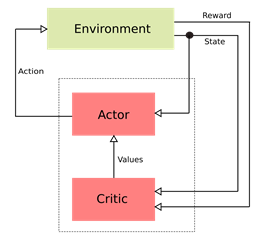
\includegraphics[width=\textwidth]{figures/RL_structure.png}
        \caption{強化學習架構圖}
        \label{fig:RL_structure}
    \end{subfigure}
    \hfill
    \begin{subfigure}[b]{0.48\textwidth}
        \centering
        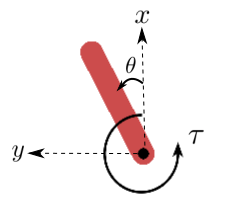
\includegraphics[width=\textwidth]{figures/pendulum.png}
        \caption{Pendulum 環境示意圖}
        \label{fig:pendulum}
    \end{subfigure}
    \caption{強化學習架構與環境示意圖}
    \label{fig:RL_and_pendulum}
\end{figure}

這裡我們使用 Pendulum-v1 這個 task 來舉例的話,環境是一個桿子,一邊固定,另一邊自由活動,我們的目標是讓桿子擺動到正上方,所以環境會給我們桿子另一個端點的 $x$ 與 $y$ 數值,以及此時的角速度 $\omega$ ,然後我們可以採取的 action 是施加的力矩 $\tau$,然後雖然我們的目標是讓桿子向上,但是同時 Reward 也提供了角速度與力矩數值的懲罰,所以這個任務的目標是,在使用少量的力矩情況下,讓桿子穩定的擺動到上方,妙的是,這裡的 Actor Network 的力矩輸出其實沒有很大的上限,也就是我們沒辦法用蠻力,把桿子往上推,所以這個任務其實是需要累積位能,然後來回擺盪兩三次內,讓桿子穩定擺動到正上方。

討論完 Enviroment 的輸入與輸出之後,我們要討論 Actor 與 Critic 的用途,Critic 的輸入是 state,輸出是 state 的價值,我們可以先想像 state 的價值是:這個狀態未來可能的 reward 總和,這裡我們可以思考一個問題,同樣是在赤壁的環境上,孔明就可以用草船獲得大量的箭矢,但是周瑜卻想不到,這就是代表 Critic 的價值估計,是需要綁定一個 Actor 的策略能力,不同的 Actor 對於相同的狀態,能發揮的價值是不同的!

\begin{figure}[h]
    \centering
    
\includegraphics[width=0.8\textwidth]{figures/Critic_value_depend_on_Actor.png}
    \caption{Critic 的價值估計與 Actor 的策略能力相關示意圖}
    \label{fig:Critic_value_depend_on_Actor}
\end{figure}

\clearpage

\subsection{How do you obtain the stochastic policy gradient and the TD error for A2C?}

那我們該怎麼建構 Critic Network 的價值觀呢? 這裡要介紹 TD error,所謂的 TD error 可以想像成我們在現在這個價值預估未來可能的 reward 總和,當作 Prediction,然後真實的走一步,得到 reward 以及新的狀態,然後再用同樣的價值網路預測 Next state 的可能 reward 總和,然後把 reward 與 next state 的預估價值加總,就是一個更貼近真實的 reward 預估值,所以我們把這個數值當作 ground truth,把 Predict 與 ground truth 計算 MSE 的 loss,透過串接每個 state 的價值,這樣 Critic Network 就可以撐起整個狀態空間的價值估計。


\begin{equation}
    loss = MSE(V(s_t), r_t + \gamma V(s_{t+1}))
\end{equation}

左邊代表我們預估的價值,右邊雖然也是估計而得,但是由於其多走了一步,得到真實的 reward ,所以是更精確的預估,這裡我們把它當作 ground truth,然後計算 MSE loss,其中 $r_t$ 是當下的 reward,$\gamma$ 是折扣因子,$V(s_{t+1})$ 是下一個狀態的價值預估,$V(s_t)$ 是當下狀態的價值預估。


但這會有個問題,就是 Reward 的傳導過慢,需要一個一個 state 的傳遞,面對這個問題,可以使用 mult-step or General Advantage Estimation (GAE) 來解決,讓 reward 可以傳遞的更遠,這裡我們使用 GAE 來解決這個問題。

接著我們回到 Actor Network 身上,由於我們的目標是讓採取的策略得到最大的期望 Reward 合:

\begin{equation}
    J(\theta) = \mathbb{E}_{\pi_\theta}[R(\tau)]
\end{equation}

其中 $\theta$ 是 Actor Network 的參數,$\pi_\theta$ 是策略函數,$R(\tau)$ 是軌跡 $\tau$ 的總獎勵,$\mathbb{E}_{\pi_\theta}$ 是在策略 $\pi_\theta$ 下的期望值。

接著我們考慮要如何做偏微分,來優化這個 Objective function:

\begin{equation}
    \nabla_\theta J(\theta) = \mathbb{E}_{\pi_\theta}[R(\tau) \nabla_\theta \log \pi_\theta(a|s) ]
\end{equation}

其中 $\nabla_\theta \log \pi_\theta(a|s)$ 是策略的對數梯度,$R(\tau)$ 是軌跡的總獎勵。這個公式告訴我們,我們可以通過對策略的對數梯度進行加權平均來估計目標函數的梯度,權重就是軌跡的總獎勵。

可是考慮到 sample 的稀疏性,在每次的 mini batch 當中,可能會有許多的策略並沒有被 sample 到,然後被 sample 的 reward 也可能總是正的,這會導致在 optimize 的過程中,「是否 sample 到」成爲了主要考量,而不是策略的好壞,這樣會導致訓練到錯誤的目標。

\begin{figure}[h]
    \centering
    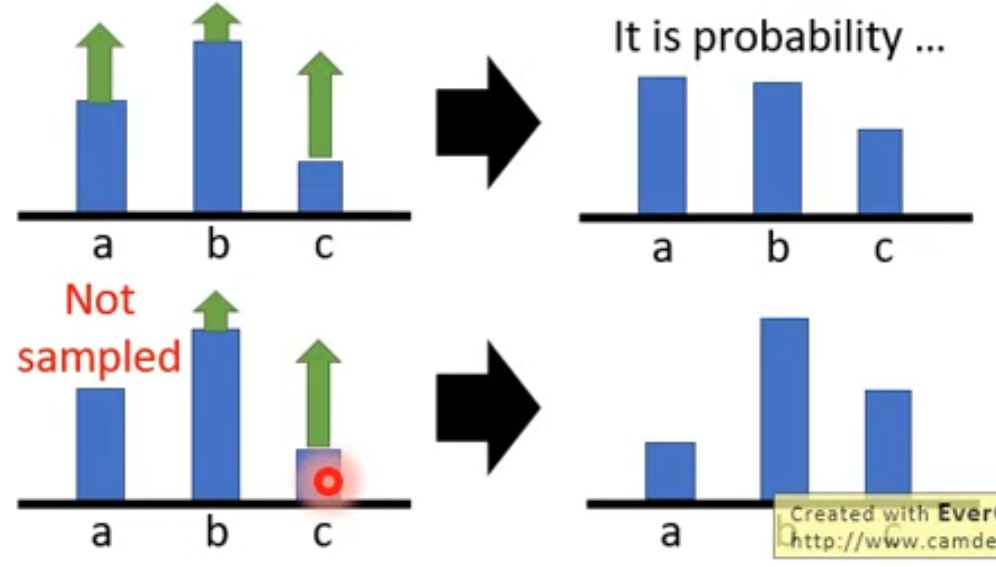
\includegraphics[width=0.8\textwidth]{figures/stochastic_issue.png}
    \caption{隨機策略梯度估計問題示意圖 \cite{lee2023drl}}
    \label{fig:stochastic_issue}
\end{figure}

如圖 \ref{fig:stochastic_issue} 所示,在隨機策略梯度的估計中,我們會遇到樣本稀疏性的問題。當我們在 mini batch 中進行採樣時,某些策略可能完全沒有被採樣到,而某些策略則可能被多次採樣。此外,被採樣到的獎勵值可能總是正值,這會導致在優化過程中,「是否被採樣到」成為主要考量因素,而不是策略本身的好壞。這種情況會導致模型訓練到錯誤的目標。

所以在不影響 Objective function 的梯度情況下,我們減去了一個 baseline ,來當作 Advantage 的估計,這樣可以減少 sampling 稀疏的影響,提高訓練的穩定性。使用優勢函數 $A(s,a)$ 來代替 $R(\tau)$:

\begin{equation}
    \nabla_\theta J(\theta) = \mathbb{E}_{\pi_\theta}[A(s,a)\nabla_\theta \log \pi_\theta(a|s) ]
\end{equation}

\begin{equation}
    A(s,a) = R(s,a) - V(s)
\end{equation}

其中 $A(s,a)$ 是優勢函數,表示在狀態 $s$ 下採取動作 $a$ 相對於平均水平的優勢$V(s)$,可以理解成這個 action 採取之後,可能比平均獲得的 Reward 總和多多少。

這就是從 valina Policy Gradient 到 Advantage Actor Critic (A2C) 的過程;Normalize 雖然很容易在數學上看起來是沒有意義的操作,但是考慮到效率與 sample 必定導致的 sample 稀疏,Normalize 是很重要的。

\subsection{How do you implement the clipped objective in PPO?}

下一個我們面對的問題就是,當 Actor 跟 Environment 互動的數據,在更新了 Actor 之後,我們就把數據丟棄了,也就是說 On-policy 的訓練方式效率非常低,雖然 PPO \cite{schulman2017ppo} 本質上仍屬於 On-policy 的範疇,但它通過引入重要性採樣和特殊的目標函數,允許使用同一批數據進行多次小批量更新,從而顯著提高了數據利用率,持續精進自己,可以想像成看偉人傳記學習的過程肯定比自己活一個人生還有效率,但是由於自己人生會採取的 action 才對自己精進最有幫助,所以我們需要結合 Off-policy 的方式看偉人傳記,然後使用自己帶入情境的方式學習,思考自己會怎麼做,來快速精進自己。

所以抽象來說,Actor loss 的目的在於,從過去的策略中抽樣,考慮自身與過去自身的 actioin 機率分布差異,然後最大化 Advantage。

\begin{equation}
    J^{\theta_{old}}(\theta) = \mathbb{E}_{\pi_{\theta_{old}}}[\frac{\pi_\theta(a|s)}{\pi_{\theta_{old}}(a|s)}A^{\theta_{old}}(s,a)]
\end{equation}

其中 J 是 Objective function,function 中的 theta 是要更新的參數,$\pi_{\theta_{old}}$ 是舊的策略,$\pi_\theta$ 是新的策略,$A^{\theta_{old}}(s,a)$ 是舊的策略下,採取動作 $a$ 的優勢函數。

但是如果偉人身處的環境與我們身處的環境差異過大,會導致我們可能本來就沒辦法做出相似的選擇,那他的傳記對我們的優化自己的幫助可能就不大,所以這裡引入了 PPO-Clip 的方式,來限制 Actor 的 action distribution 不要差異過大。


\begin{equation}
    L^{CLIP}(\theta) = \hat{\mathbb{E}}_t[\min(r_t(\theta)A_t, \text{clip}(r_t(\theta), 1-\epsilon, 1+\epsilon)A_t)]
\end{equation}

其中 $r_t(\theta)$ 是新舊策略的比率:

\begin{equation}
    r_t(\theta) = \frac{\pi_\theta(a_t|s_t)}{\pi_{\theta_{old}}(a_t|s_t)}
\end{equation}

這個公式的核心思想是:如果新策略與舊策略的差異太大,我們就限制更新的幅度,避免策略更新過大導致訓練不穩定。具體來說,當優勢值為正時,我們希望增加該動作的機率,但不會超過 $1+\epsilon$ 倍;當優勢值為負時,我們希望減少該動作的機率,但不會低於 $1-\epsilon$ 倍。這樣可以確保策略更新的穩定性。

那為什麼要用 min 又用 clip 呢? 這裡我們使用表格討論:

\begin{table}[h]
    \centering
    \begin{tabular}{|c|c|c|c|}
        \hline
        & $r < 1-\epsilon$ & $1-\epsilon \leq r \leq 1+\epsilon$ & $r > 1+\epsilon$ \\
        \hline
        $A > 0$ & $rA$ & $rA$ & $(1+\epsilon)A$ \\
        \hline
        $A < 0$ & $(1-\epsilon)A$ & $rA$ & $rA$ \\
        \hline
    \end{tabular}
    \caption{PPO-Clip 在不同情況下的更新幅度}
    \label{tab:ppo_clip}
\end{table}

我們不要讓模型過度樂觀,如(1-3, 2-1),但是如果當模型錯誤的降低了具有優勢的 action 機率時,我們要給予實際的懲罰,如 (1-1 與 2-3),總而言之,PPO-Clip 限制了有利的更新,卻保持對不利的更新的敏感,未慮勝 先慮敗!


\subsection{How do you obtain the estimator of GAE?}

在解決完數據使用效率上的問題之後,我們仍然在效率上面尋求突破,GAE 想要解決的問題就是,更穩定的估計 Advantage。

在估計 Advantage 傳統方法有兩個可以使用,一個是 Monte Carlo (MC) 的方法,一個是 TD 的方法,Monte Carlo 的方法是直接估計整個軌跡的 reward 總和,而 TD 的方法是估計下一個 state 的價值,然後用這個價值來估計 Advantage。 MC 的問題很明顯就是要等遊戲全部玩完之後,可以得到一個完整的軌跡,雖然準確率高,但是不穩定,然而 TD 的方法,可以使用每一個 Reward 來更新模型,相對於完整軌跡,穩定性更加,因為 TD 所涉及的隨機性,僅僅只有一個 Action,但這會有問題就是,Reward 的傳遞過慢,需要一個一個 state 的傳遞,所以 GAE 的出現,就是為了平衡兩者的優缺點。

GAE 透過加權平均未來的 Reward 來提供一個更好的模型優化方向,讓 Reward 可以把優化的訊號傳遞到更前面的 Action 選擇上,另外利用 $\lambda$ 來遞減較遠未來的 Reward 的權重,若以 0.95 舉例:當未來 60 步之後得到的 Reward 權重只剩下 5\% 以下,這讓模型可以在穩定性與準確性之間做平衡,看我們需要考慮的 Task 的步數距離來調整 $\lambda$ 的值。

\begin{equation}
    A_t = \sum_{i=0}^{\infty} \lambda^{i} \delta_{t+i}
\end{equation}

在實作上,我們可以用 $O(N)$ 的時間複雜度,從後面往前計算 GAE 的值,這樣可以避免每次都重新計算整個軌跡的 Reward 總和,這樣可以節省計算時間,提高訓練效率,然後最後在把 GAE 的數值全部做 Normalize,讓模型在更新的時候,不會逞罰沒有被抽樣的策略,而是懲罰表現不佳的策略。

這裡可以再討論一下 critic 的 loss 計算,在確立了 GAE 的策略之後,具體而言,我是使用 過去的 value + action 的 advantage 來得到 target value,然後使用當前的 critic 得到當前的 state 的 value,然後計算兩者的 MSE 來得到 actor 的 loss,我想可以抽像成,現在我們有一個 action ,得到了 reward,這個新的資訊,是過去模型不具備的,我們需要讓 critic 的 value 學習這個 action 之後,所帶來的新的價值判斷,所以 target value 是過去的 value + advantage ,然後 predict value 是當前的 value,這樣可以讓模型在估計 state 的價值時,多考慮一個新的策略帶來的價值影響。



\subsection{How do you collect samples from the environment?}

首先我使用 Rollout 的方式,先採集指定 env step 的數據,然後計算 GAE 的值,接著根據 batch size 的大小製作 dataloader,然後傳回給 update 的過程使用,來實現小批樣本的多次更新,提升樣本的使用效率。

這裡我是有查到可以同時開啟多個環境收集數據,但是我當初在規劃 code 的架構時,就已經預設只有一個 env,所以有大量的 code 需要重新撰寫與測試,這讓我覺得非常無力,所以最後我是使用單台電腦,多開幾個 training 的 process ,來單次測試大量的超參數,來彌補我 sample data 效率上的問題。

\clearpage
\subsection{How do you enforce exploration (despite that both A2C and PPO are on-policy RL methods)?}

在 A2C 與 PPO 當中,我們是使用 Actor 輸出一個高斯分佈,然後在訓練的時候從這個分布中抽樣 action,然後 test 的時候就使用 mean value 當作 action,藉此保證了 Actor 的探索能力,然而在訓練的過程中,探索勢必會帶來不穩定,導致 Reward 的懲罰,所以模型在學習的過程中,天然的會讓 std 變小,來降低不確定性,所以探索能力就坍塌了,所以我們需要加入 Entropy 來計算 Actor 輸出的高斯分佈的熵值,來保證探索能力。

所以在 A2C 與 PPO 當中,是依靠模型內部的隨機性來探索,而不像是 Q Learning 的時候,會先才取隨機的行動,然後才開始訓練模型。

\begin{equation}
    L_{entropy} = -\mathbb{E}_{\pi_\theta}[log(\pi_\theta(a|s))]
\end{equation}


\subsection{How do you use Weight \& Bias to track model performance and the loss values (including actor loss, critic loss, and the entropy)?}


我使用 Wandb 來確立 Entropy 真的很重要的,因為 Entropy 的 Reward 都一直非常低,所以起初我是不願意使用 Entropy 的,但是當我看到 Critic Value 開始上不去的時,與 reward 開始停滯是同樣時刻,以及 action 的 Entropy 也剛好陷入了停滯區,這三個時刻串在一起,就讓我知道,Entropy 真的突破 2000 分的關鍵。

\begin{figure}[h]
    \centering
    \begin{subfigure}[b]{0.8\textwidth}
        \centering
        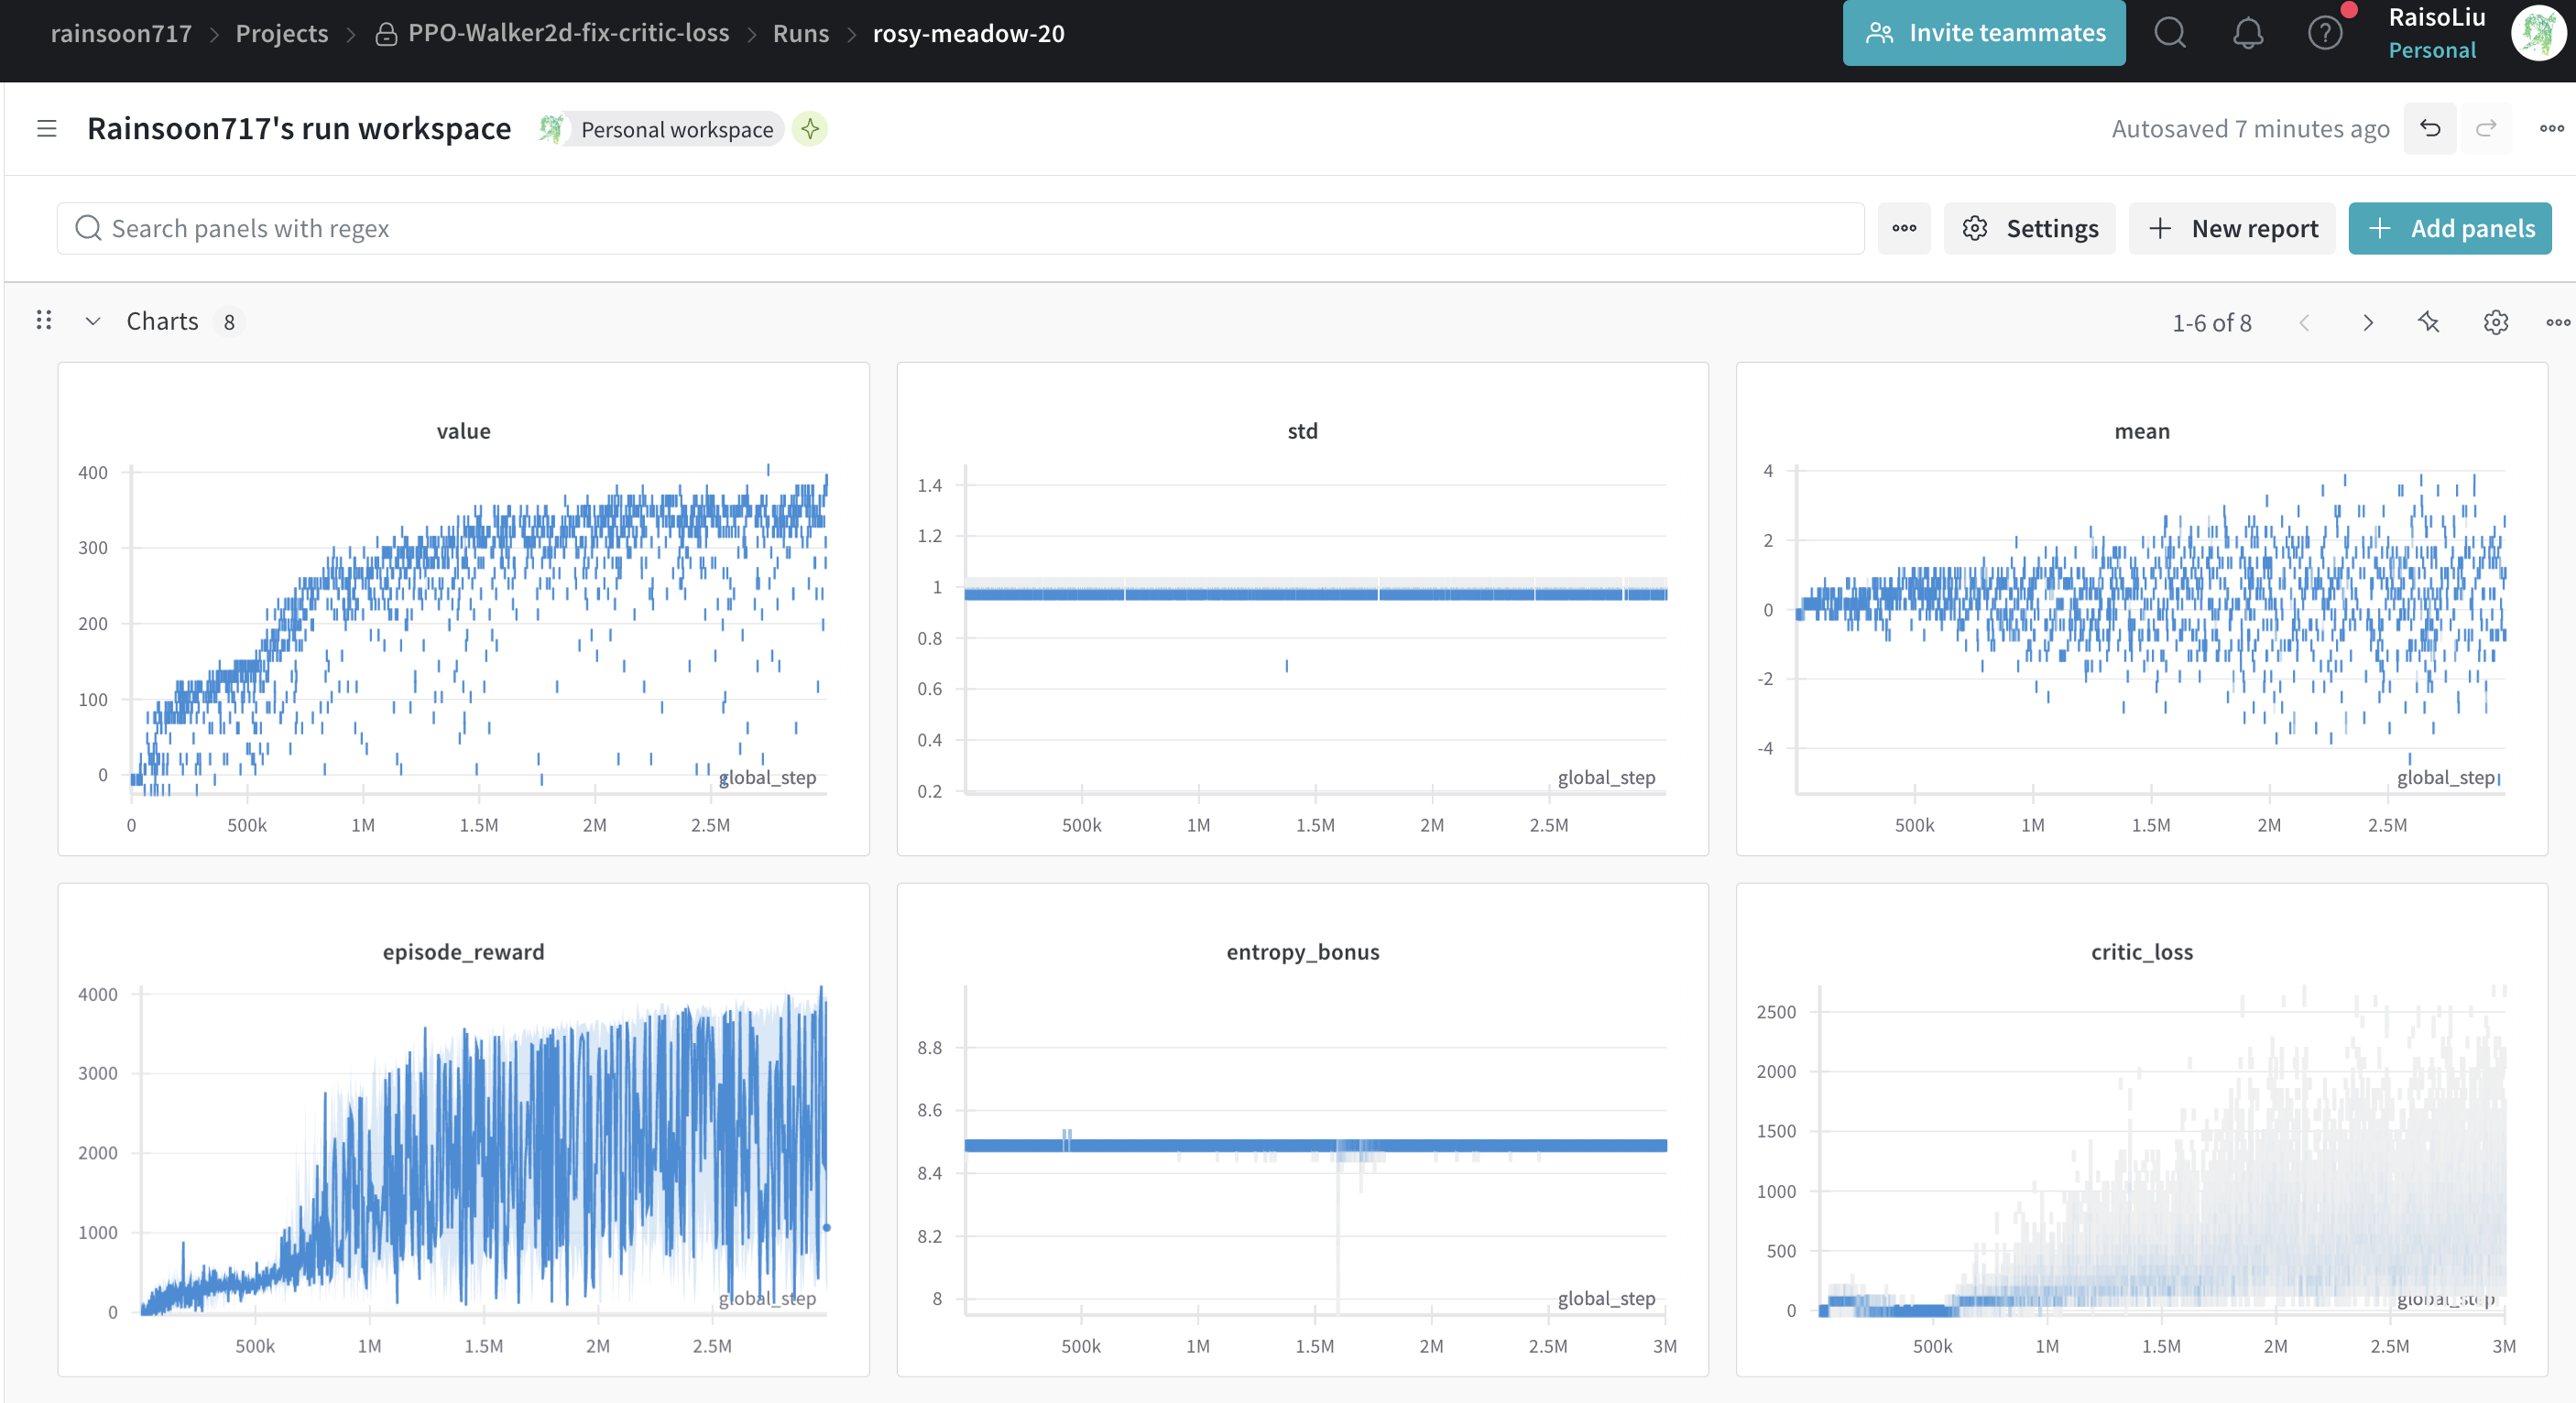
\includegraphics[width=\textwidth]{figures/wandb_case1.png}
        \label{fig:wandb_case1}
    \end{subfigure}
    \hfill
    \begin{subfigure}[b]{0.8\textwidth}
        \centering
        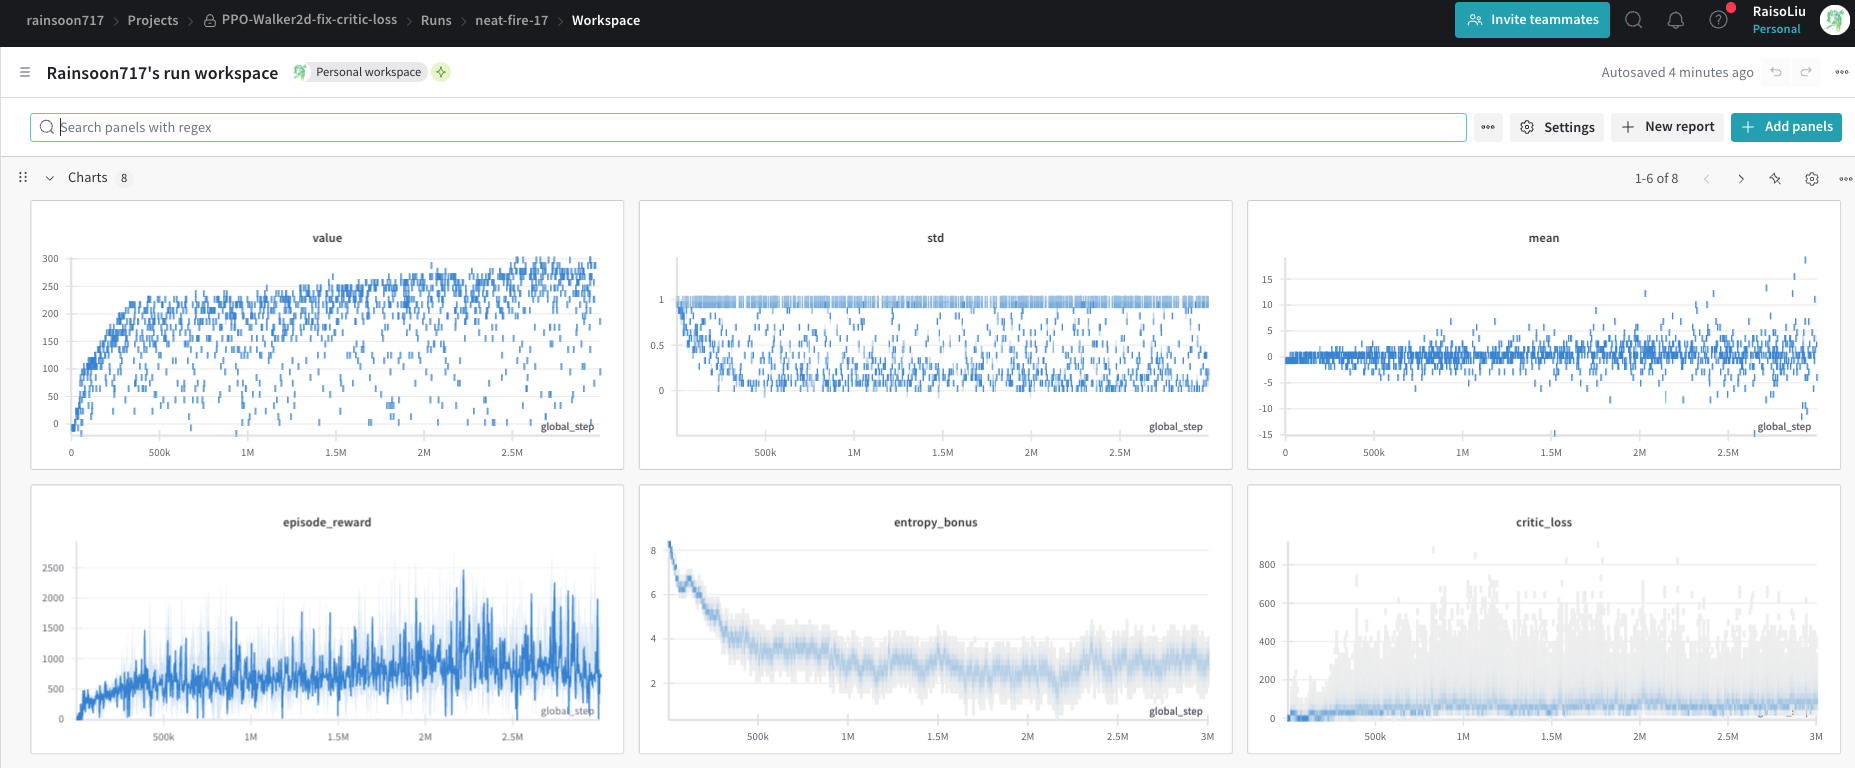
\includegraphics[width=\textwidth]{figures/wandb_case2.png}
        \label{fig:wandb_case2}
    \end{subfigure}
    \caption{Entropy 與模型表現的關係圖}
    \label{fig:wandb_cases}
\end{figure}

但是代價是,單次訓練的 model size 不到 1MB ,但是 log 到達了 22GB。